%Every piece of package I've acumulated over the last years
%%%%%%%%%%%%%%%%%%%%%%%%%%%%%%%%%%%%%%%%%%%%%%%%%%%%%%%%%%%%%%%%%%%%%%%%%%%%%%%%%%%%%%%%%%%%%%
\documentclass[a4paper,12pt]{article}
\usepackage[utf8]{inputenc}
\usepackage{imakeidx}
\usepackage{graphicx}
\usepackage{float}
\usepackage{amsmath}
\usepackage[backend=bibtex,style=verbose]{biblatex}
\bibliography{bibliography}
\usepackage{csquotes}
\usepackage{tcolorbox}
\usepackage{multirow}
\usepackage{caption}
\usepackage{afterpage}
\usepackage[margin=1in]{geometry}
\usepackage[english,spanish]{babel}
\usepackage{tikz}
\usepackage{mwe}
\usepackage{circuitikz}
\usepackage{subcaption}
%%%%%%%%%%%%%%%%%%%%%%%%%%%%%%%%%%%%%%%%%%%%%%%%%%%%%%%%%%%%%%%%%%%%%%%%%%%%%%%%%%%%%%%%%%%%%%
\begin{document}
\title{Evaluación Continua de Mecánica II\\ Tema 1}
\author{Gabriel D'Andrade Furlanetto}
\maketitle 

\section{Circuitos LRC acoplados}
En este problema, analizaremos el circuito representado en la Figura \ref{circ} 

\begin{figure}[H]
  \centering
  \caption{Circuito a ser analizado}
  \label{circ}
  \begin{circuitikz}[american voltages]
    \draw
    (0,0) to  [C, l=$C$](2,0)
    to [C, l=$C$] (4,0) 
    to [L, l=$L$] (4,-2)
    to [R, l=$R$] (2,-2)
    to [R, l=$R$] (0,-2)
    to [L, l=$L$] (0,0)
    (2,0) to [L, l=$L$] (2,-2);
  \end{circuitikz}
\end{figure}


\subsection*{a) Escribe las ecuaciones de Kirchoff del circuito y encontra los modos y frecuencias normales.}

Para escribir las ecuaciones de Kirchoff, tenemos que analizar las corrientes utilizando la Ley de Corrientes de Kirchoff, y las tensiones, utilizando la Ley de Voltajes de Kirchoff. El primero es trivial, y está hecho en la Figura \ref{k1}. Para el segundo, utilizaremos las mallas en la Figura \ref{k2}.

\begin{figure}[H]
    \centering
    \begin{minipage}{0.45\textwidth}
        \centering
        \begin{otherlanguage}{english}
        \begin{circuitikz}[american voltages]
          \draw node at (0.45, 0.45) {$I_1$};
          \draw[->] (0.15,0.15)-- (0.75,0.16);
          \draw node at (2.45, 0.45) {$I_2$};
          \draw[->] (2.15,0.15)-- (2.75,0.16);
          \draw node at (1.2, -1) {$I_1-I_2$};
          \draw[->] (1.75,-0.50)-- (1.75,-1.5);
          \draw
          (0,0) to  [C, l=$C$](2,0)
          to [C, l=$C$] (4,0) 
          to [L, l=$L$] (4,-2)
          to [R, l=$R$] (2,-2)
          to [R, l=$R$] (0,-2)
          to [L, l=$L$] (0,0)
          (2,0) to [L, l=$L$] (2,-2);
    \end{circuitikz}
    \end{otherlanguage}
        \caption{Análisis de corrientes}
        \label{k1}
    \end{minipage}\hfill
    \begin{minipage}{0.45\textwidth}
    \begin{otherlanguage}{english}
        \centering
        \begin{circuitikz}[american voltages]
          \draw node at (1,-1) {1};
          \draw node at (3,-1) {2};
          \draw[thick, <-] (1.65,-1) arc (0:320:0.6);
          \draw[thick, <-] (3.65,-1) arc (0:320:0.6);
          \draw
            (0,0) to  [C, l=$C$](2,0)
            to [C, l=$C$] (4,0) 
            to [L, l=$L$] (4,-2)
            to [R, l=$R$] (2,-2)
            to [R, l=$R$] (0,-2)
            to [L, l=$L$] (0,0)
            (2,0) to [L, l=$L$] (2,-2);
    \end{circuitikz}
    \end{otherlanguage}
        \caption{Análisis de mallas}
        \label{k2}
  \end{minipage}
\end{figure}

 Tendremos, finalmente, dos ecuaciones utilizando que $\sum V = 0$ para una malla cerrada. Como $I = \dot{Q}$, seremos capaces de escribir las ecuaciones para la primera y segunda malla, respectivamente:
  \begin{equation}
  \label{eq1}
  \begin{aligned}
  \frac{1}{C} Q_1 + R \dot{Q}_1 + L\ddot{Q}_1 + L(\ddot{Q}_1 - \ddot{Q}_2)) = 0\\
  \frac{1}{C} Q_2 + R \dot{Q}_2 + L\ddot{Q}_2 - L(\ddot{Q}_1 - \ddot{Q}_2)) = 0
  \end{aligned}
  \end{equation}

A este sistema de ecuaciones diferenciales lineales de orden 2 no será posible aplicar las técnicas estándar que desarrollamos durante el curso, ya que tenemos términos con dependencia en las velocidades, o sea, tenemos oscilaciones amortiguadas.

De esta manera, podemos mirar fijamente el Sistema \eqref{eq1} y percibir que si sumamos o tomamos la diferencia de las ecuaciones, podremos trivialmente encontrar unas coordenadas normales (esto es, desacopladas). Es decir, podemos escribir nuestras ecuaciones como:

$$ \frac{1}{C} (Q_1 + Q_2) + R (\dot{Q}_1 + \dot{Q}_2)  + L (\ddot{Q}_1 + \ddot{Q_2})=0 \qquad \text{(Suma)}$$
$$\frac{1}{C} (Q_1 - Q_2) + R (\dot{Q}_1 - \dot{Q}_2) + 3L (\ddot{Q}_1 - \ddot{Q}_2) = 0 \qquad \text{(Sustracción)}$$

Escrito de esa manera, no es un salto de lógica muy grande hacer el siguiente cambio de coordenadas:

\begin{equation}
  \begin{aligned}
    \eta = Q_1 + Q_2 \\
    \xi = Q_1 - Q_2 
  \end{aligned} 
\end{equation}

De manera que tendremos dos osciladores amortiguados desacoplados:

\begin{equation}
\label{coords1}
  \begin{aligned}
    \ddot{\eta} + 2\left(\frac{R}{2L}\right) \dot{\eta} + \left(\sqrt{\frac{1}{CL}}\right)^2 \eta = 0 \\
    \ddot{\xi} + 2\left(\frac{R}{6L}\right) \ddot{\xi} + \left(\sqrt{\frac{1}{3CL}}\right)^2 \xi = 0
  \end{aligned}
\end{equation}

Y podemos encontrar la solución para $\eta$ y $\xi$ por los métodos estándar:
\begin{equation}
\label{coords1}
  \begin{aligned}
    \eta(t) = e^{-\frac{R}{2L}t}\left[A_1 e^{\sqrt{\left(\frac{R}{2L}\right)^2 -\frac{1}{CL}}t} + A_2e^{-\sqrt{\left(\frac{R}{2L}\right)^2 -\frac{1}{CL}}t}\right]\\
    \xi(t) = e^{-\frac{R}{6L}t}\left[A_1 e^{\sqrt{\left(\frac{R}{6L}\right)^2 -\frac{1}{3CL}}t} + A_2e^{-\sqrt{\left(\frac{R}{6L}\right)^2 -\frac{1}{3CL}}t}\right]
  \end{aligned}
\end{equation}

Que no ilumina básicamente nada de nuestro problema.\footnote{Las soluciones tienen más sentido después de ser determinado el régimen de amortiguación}. 

No obstante, solo tendrá sentido hablar de frecuencias normales para el régimen de amortiguamiento débil, ya que es el único que de hecho oscila, y serán definidas por:

\begin{equation}
  \label{eta}
  \omega_{\eta} = \sqrt{\frac{1}{CL} - \left(\frac{R}{2L}\right)^2}
\end{equation}
\begin{equation}
  \label{xi}
  \omega_{\xi} = \sqrt{\frac{1}{3CL} - \left(\frac{R}{6L}\right)^2}
\end{equation}

Es importante mencionar que, una vez encontrados $\eta(t)$ y $\xi(t)$, podemos trivialmente obtener expresiones para $Q_{1}$ y $Q_2$ de la ecuación \eqref{coords1}\footnote{No será muy útil o instructivo hacerlo para las ecuaciones generales de \eqref{eta} y \eqref{xi}, entonces lo haremos solo para el caso particular del apartado siguiente.}:

\begin{equation}
  \begin{aligned}
  \label{equonts}
    Q_1(t) = \frac{\eta(t) + \xi(t)}{2}\\
    Q_2(t) = \frac{\eta(t) - \xi(t)}{2} 
  \end{aligned}
\end{equation}

Finalmente, no es mala idea hacer las analogías que este sistema electrónico tiene a sistemas mecánicos explicita: La decisión de discutir la carga $Q_{i}$ en los capacitores\footnote{Y no corrientes, como se hace usualmente en electrónica} no fue una trivialidad, sino algo que hecho adrede para hacer una conexión estrecha con las coordenadas generalizadas $q_i$. 

De hecho, si se omitiera la primera página de este documento, sería bastante razonable esperar que estuviera resolviendo el problema 25 de la lista de problemas, un oscilador acoplado con un pistón viscoso, representado en la Figura \ref{amort}
\begin{figure}
  \centering
  \caption{Problema 25: Masas-muelles acoplados con pistón viscoso.}
  \label{amort}
  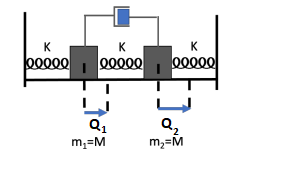
\includegraphics[width=0.5\textwidth]{amort.jpg}
\end{figure}

Fundamentalmente, los métodos de la mecánica clásica no comienzan y acaban en posiciones generalizadas y momentos canónicos, y este problema lo ilustra un poco.

\subsection*{b) Discute los regímenes de amortiguación del circuito. Escribe la solución para el caso particular de $6L = CR^2$}

Algunas generalidades de los regímenes de amortiguación fueron discutidas en la sección anterior, pero fundamentalmente estará dado para cada modo normal por el signo de las cantidades:

$$\Delta_\eta = \left(\frac{R}{2L}\right)^2 - \frac{1}{CL}$$
$$\Delta_\xi = \left(\frac{R}{6L}\right)^2 - \frac{1}{3CL}$$

Si son positivas, tendremos el régimen de sobre-amortiguamiento. Si son 0, tendríamos un amortiguamiento crítico, y si son negativas, tendremos el amortiguamiento débil. Para el caso de $R^2 =\frac{6 L }{C} $, tendremos que:

\begin{equation}
  \Delta_\eta = \frac{R^2}{4 L^2} - \frac{1}{CL} = \frac{6L}{4 L^2 C} - \frac{1}{CL} = \frac{1}{CL} \left(\frac{3}{2} - 1\right) > 0
\end{equation}

Que significa que la coordinada $\eta$ estará sobreamortiguado. Para el otro,

\begin{equation}
  \Delta_\xi = \frac{R^2}{36L^2} - \frac{1}{3CL} = \frac{6 L}{36 L^2 C} - \frac{1}{3CL} = \frac{1}{CL} \left(\frac{1}{6} - \frac{1}{3}\right) < 0
\end{equation}

O sea, la coordinada $\xi$ estará en el régimen de amortiguación débil.

De esta manera, podemos escribir las ecuaciones para los dos:

\begin{equation}
\eta (t) =   e^{-\frac{R}{2L} t}  \left[A_1 e^{\sqrt{\frac{1}{2CL}} t} + B_1 e^{-\sqrt{\frac{1}{2CL}} t}\right]
\end{equation}


\begin{equation}
\xi(t) = e^{-\frac{R}{6CL} t}  A_2\cos{\left(\frac{1}{6CL} t + B_2\right)} 
\end{equation}

Por lo que tenemos que la solución general de nuestro sistema será\footnote{Se ha absorbido el factor de $\frac{1}{2}$ de la ecuación \eqref{equonts} a las constantes. Al final, una constante partido dos es otra constante.}:

\begin{equation}
  \begin{aligned}
     Q_1(t)& = \eta(t) + \xi(t) \\&= e^{-\frac{R}{2L} t}  \left[A_1 e^{\sqrt{\frac{1}{2CL}} t} + B_1 e^{-\sqrt{\frac{1}{2CL}} t}\right] + e^{-\frac{R}{6CL} t}A_2\cos{\left(\frac{1}{6CL} t + B_2\right)}  
  \end{aligned}
\end{equation}

\begin{equation}
\begin{aligned}
    Q_2(t) &= \eta(t) - \xi(t) \\&= e^{-\frac{R}{2L} t}  \left[A_1 e^{\sqrt{\frac{1}{2CL}} t} - B_1 e^{-\sqrt{\frac{1}{2CL}} t}\right] -e^{-\frac{R}{6CL} t} A_2\cos{\left(\frac{1}{6CL} t + B_2\right)}
\end{aligned}
\end{equation}

Para la corriente, tenemos que derivar estas expresiones. La expresión no son elegantes, pero al final, tendremos que:

\begin{equation}
\begin{aligned}
  I_1(t) =& e^{-\frac{R}{2L} t}  \left[A_1\left(\frac{1}{2CL}- \frac{R}{2L}\right) e^{\sqrt{\frac{1}{2CL}} t} - \left(\frac{1}{2CL}+ \frac{R}{2L}\right)B_1 e^{-\sqrt{\frac{1}{2CL}} t}\right] - A_2 e^{-\frac{R}{6CL} t} \beta\cos{\left(\frac{1}{6CL} t + B_2\right)}\\& + \frac{1}{6CL}\sin{\left(\frac{1}{6CL} t + B_2\right)}
\end{aligned}
\end{equation}

\begin{equation}
\begin{aligned}
  I_2(t) =& e^{-\frac{R}{2L} t}  \left[A_1\left(\frac{1}{2CL}- \frac{R}{2L}\right) e^{\sqrt{\frac{1}{2CL}} t} - \left(\frac{1}{2CL}+ \frac{R}{2L}\right)B_1 e^{-\sqrt{\frac{1}{2CL}} t}\right] + A_2 e^{-\frac{R}{6CL} t} \beta\cos{\left(\frac{1}{6CL} t + B_2\right)}\\& + \frac{1}{6CL}\sin{\left(\frac{1}{6CL} t + B_2\right)}
\end{aligned}
\end{equation}

\pagebreak

\section{ Partículas de masas m en barras fijas con ángulo constante de 2$\alpha$ entre si conectadas con muelles.}
En este problema, analizaremos el sistema mecánico representado en la Figura \ref{2nd}.
\begin{figure}
  \centering
  \caption{Representación del Problema 2}
  \label{2nd}
  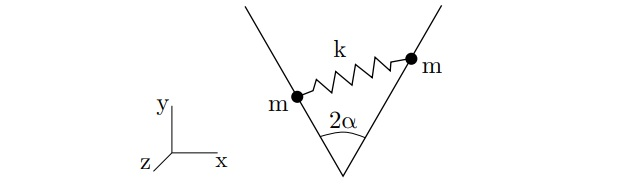
\includegraphics{2.jpg}
\end{figure}

\subsection*{a) Supongamos que hay un campo gravitatorio $g$ en la dirección negativa del eje $y$. Calcula el Lagrangiano, posición de equilibrio, modos y frecuencias normales.}

Para este problema, lo más conveniente es utilizar la distancia del vértice como las coordenadas generalizadas, que llamaremos de $\rho_{1}$ y $\rho_2$. Por algunas relaciones trigonométricas básicas, representadas en la Figura \ref{repr}, tendremos que:

\begin{equation}
  \begin{aligned}
    x_1 = \rho_1 \sin{(\alpha)}\\
    y_1 = \rho_1 \cos{(\alpha)}
  \end{aligned}
\end{equation}
\begin{equation}
  \begin{aligned}
    x_2 = \rho_2 \sin{(\alpha)}\\
    y_2 = \rho_2 \cos{(\alpha)}
  \end{aligned}
\end{equation}

\begin{figure}[h!]
  \centering
  \caption{Representación esquemática del sistema}
  \label{repr}
  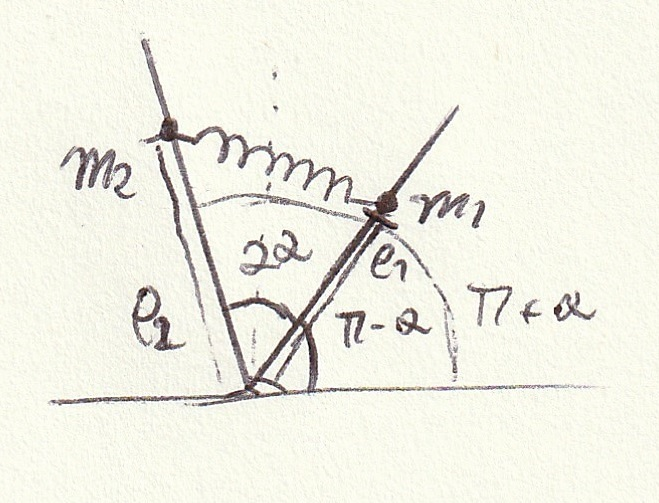
\includegraphics{repr.jpg}
\end{figure}

\subsubsection*{Lagrangiano}
Trivialmente podemos calcular la energía cinética, que nos saldrá:

\begin{equation}
  T = \frac{1}{2}m (\dot{\rho_1} + \dot{\rho_2})
\end{equation}
Por la presencia de la gravedad, sabemos que la energía potencial tendrá dos términos, uno gravitacional que va a depender de $y_i$ y otro elástico que dependerá de $D$, la distancia entre las masas. Por la ley de cosenos podemos trivialmente calcular esta distancia:

$$D =\sqrt{\rho_1^2 + \rho_2^2 -2\rho_1\rho_2\cos{(2\alpha)}} $$


La energía potencial estará dada por:

$$U = \frac{1}{2}k(D-l_0)^2 + mgy_1+mgy_2 = \frac{1}{2}k \left(\sqrt{\rho_1^2 + \rho_2^2 -2\rho_1\rho_2\cos{(2\alpha)}} - l_0\right)^2 + mg\cos{(\alpha)}\left(\rho_1+\rho_2\right)$$




O sea, nuestro Lagrangiano será:

\begin{equation}
  L = \frac{1}{2}m (\dot{\rho_1} + \dot{\rho_2}) - \frac{1}{2}k (\sqrt{\rho_1^2 + \rho_2^2 -2\rho_1\rho_2\cos{(2\alpha)}} - l_0)^2 + mg\cos{(\alpha)}\left(\rho_1+\rho_2\right)
\end{equation}

\subsubsection*{Equilibrio}

No es trivial obtener las posiciones de equilibrio de este sistema, pero utilizaremos dos hechos para hacerlo: 1) En el equilibrio, la derivada con respeto a las coordenadas es 0. 2) Por simetría, el equilibrio de este problema requiere $\rho_{1eq} = \rho_{2 eq} =\rho_{eq}$\footnote{Si el argumento de simetría no es suficiente, tomando los dos parciales y haciéndolos 0 te dará un sistema de ecuaciones donde una de las soluciones será esta condición.}. De esta manera, somo conducidos a:

$$\left(\frac{\partial U}{\partial \rho_1}\right)_{\rho_1 = \rho_2 = \rho_{eq}} = 2(2\rho_{eq} \sin(\alpha)-l_0)\frac{k(2-\cos(2a))}{\sin(\alpha)} + mg\cos{(\alpha)} = 0$$

De manera que:

\begin{equation}
\label{eq}
\rho_{eq} = \frac{l_0}{2\sin(\alpha)} - \frac{mg \cos{\alpha}}{4k(2-\cos{(2\alpha)})} 
\end{equation}

\subsubsection*{Autofrecuencias}
Si cambiamos de coordenadas, de modo que $\bar{\rho}_{i} = \rho_{i} - \rho_{i eq} $, será trivial extraer las matrices de masa y de rigidez\footnote{En coordenadas de equilibrio, hechas las expansiones de Taylor, \textit{siempre} se eliminan todos los términos de orden diferente que 2 del potencial, y como la matriz de rigidez es estrictamente los coeficientes de estos términos, no será más que un ejercicio en encontrar estos términos cuadráticos.}, que serán respectivamente: 
\begin{equation}
  M = m\begin{pmatrix}
    1&0\\0&1
  \end{pmatrix}
\end{equation}

\begin{equation}
  K = k\begin{pmatrix}
    1&-\cos{(2\alpha)}\\-\cos{(2\alpha)}&1
  \end{pmatrix}
\end{equation}

Para encontrar las autofrecuencias, vamos a utilizar la ecuación secular (y llamaremos $\omega^2 = \lambda$ por conveniencia). De esta manera, tendremos que:
\begin{equation}
\det\left(K - M \lambda\right) = \begin{vmatrix}
  k-m\lambda & k\cos{2\alpha}\\ k\cos{2\alpha}&k-m\lambda
\end{vmatrix}=0
\end{equation}

Una ecuación bastante sencilla de resolver, de donde encontraremos que:

$$\lambda = \frac{1}{m} (k \pm k\cos{2\alpha}) = \frac{k}{m} (1\pm \cos{2\alpha})$$

De modo que las frequencias normales son:
\begin{equation}
  \begin{aligned}
  \omega_0 = \sqrt{ \frac{k}{m} (1 - \cos{2\alpha})}\\
  \omega_1 = \sqrt{ \frac{k}{m} (1 + \cos{2\alpha})}
  \end{aligned}
\end{equation}
\subsubsection*{Caso límite: Masas libres}

Antes de sacar los modos normales, que a priori pueden ser nada-triviales, es informativo ver si nuestro sistema complejo nos da las ecuaciones correctas para el caso más sencillo. Concretamente, analizaremos el caso de $2\alpha = \pi$, que corresponde a un sistema bastante conocido de dos masas libres acopladas entre si, reprentado en la figura \ref{masamuelle}

\begin{figure}[h]
  \centering
  \caption{Límite del problema cuando $2\alpha = \pi$}
  \label{masamuelle}
  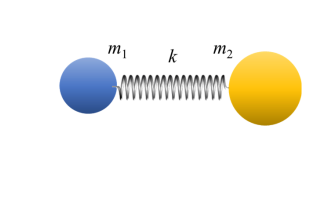
\includegraphics[width=0.5\textwidth]{masamuelle.png}
\end{figure}

Como $\cos{\pi} = -1$, llegaremos de nuestras ecuaciones a dos frecuencias normales, $\omega_0 = 0$ y $\omega_1 = \sqrt{2\frac{k}{m}}$. La frecuencia de 0 puede ser preocupante, pero físicamente corresponde al hecho de que tenemos una simetría espacial. De cualquier manera, esas son exactamente las frecuencias de ese oscilador, algo que cualquiera puede verificar trivialmente. Por buen camino vamos. 

\subsubsection*{Modos normales}

Para el primer modo, tomaremos $\lambda_0 =  \frac{k}{m} (1 - \cos{2\alpha})$ y lo pondremos en la ecuación:

$$(K-\lambda_0 M)\eta_0 = 0$$
\begin{equation*}
  \begin{pmatrix}
    k - k(1-\cos{2\alpha}) & -kcos{2\alpha}\\
    -kcos{2\alpha} & k - k (1-cos{2\alpha})
  \end{pmatrix}
  \begin{pmatrix}
    \eta_{01}\\
    \eta_{02}
  \end{pmatrix} = \begin{pmatrix}
    0 \\ 0
  \end{pmatrix}
\end{equation*}
\begin{equation*}
  \begin{pmatrix}
      k\cos{2\alpha} & -kcos{2\alpha}\\
    -kcos{2\alpha} &  kcos{2\alpha}
  \end{pmatrix}
  \begin{pmatrix}
    \eta_{01}\\
    \eta_{02}
  \end{pmatrix} = \begin{pmatrix}
    0 \\ 0
  \end{pmatrix}
\end{equation*}

Ecuación esta trivial de resolver, 
\begin{equation}
  \eta_0 = \begin{pmatrix}
    1\\1
  \end{pmatrix}
\end{equation}

Similarmente, podemos encontrar al otro modo normal:
\begin{equation}
  \eta_1 = \begin{pmatrix}
    1\\-1
  \end{pmatrix}
\end{equation}

Que podemos reescribir en términos de las coordenadas de equilibrio:

\begin{equation}
  \begin{aligned}
  \label{etas}
  \eta_0 = \bar{\rho}_1 + \bar{\rho}_2\\
  \eta_1 = \bar{\rho}_1 - \bar{\rho}_2
  \end{aligned}
\end{equation}

Estos modos corresponden a los usuales simétrico/anti-simétrico de los problemas con dos grados de libertad, que es lo  que se esperaría. 
\subsection*{b) De la posición inicial, se las da velocidad $v_0$ a una de las masas. Calcula la posición de las masas con respeto al tiempo. Si $mg = kl_0$, determina el valor mínimo de $v_0$ para que el muelle sea perpendicular a alguna de las barras.}

\subsubsection*{Posición en función del tiempo}

Este problema es equivalente a las condiciones iniciales $\bar{\rho}_{1}(0) =\bar{\rho}_{2}(0) = \dot{\bar{\rho}_{2}}(0) = 0$ y $\dot{\bar{\rho_1}}(0) = v_{0}$. Equivalentemente, si ponemos estas condiciones en la ecuación \eqref{etas} esto sería tomar $\eta_{0}(0) = \eta_1{1}(0) = 0$ y $\dot{\eta}_{0}(0) = \dot{\eta}_1{1}(0) = v_0$. Sabemos que la expresión general para estos modos será:

\begin{equation*}
  \begin{aligned}
  \eta_0 (t)= A_0 \cos(\omega_0 t) + B_0 \sin(\omega_0 t)
  \eta_1 (t) = A_1 \cos(\omega_1 t) + B_1 \sin(\omega_1 t)
  \end{aligned}
\end{equation*}

O sea, tendremos que:
\begin{equation*}
  \begin{aligned}
  \eta_0 (0)= A_0 \cos(\omega_0 0) + B_0 \sin(\omega_0 0) = A_0 = 0
  \eta_1 (0) = A_1 \cos(\omega_1 0) + B_1 \sin(\omega_1 0) = A_1 = 0
  \end{aligned}
\end{equation*}

\begin{equation*}
  \begin{aligned}
  \dot{\eta}_0 (0)= B_0 \omega_0\cos(\omega_0 0) = B_0 \omega_0 = v_0
  \dot{\eta}_1 (0) = B_1\omega_1 \cos(\omega_1 0) = B_1\omega_1 = v_0
  \end{aligned}
\end{equation*}

De manera que:

\begin{equation}
  \begin{aligned}
  \eta_0 (t) = \frac{v_0}{\omega_0} \sin(\omega_0 t)
  \eta_1 (t) = \frac{v_0}{\omega_1} \sin(\omega_1 t)
  \end{aligned}
\end{equation}

Finalmente, podemos extraer de la ecuación \eqref{etas} que:
\begin{equation}
  \bar{\rho_1}(t) = \frac{\eta_0 (t) + \eta_1(t)}{2} =\frac{v_0}{2\omega_0} \sin(\omega_0 t) +\frac{v_0}{2\omega_1} \sin(\omega_1 t)
\end{equation}
\begin{equation}
  \bar{\rho_2} (t)= \frac{\eta_0 (t) - \eta_1(t)}{2} =\frac{v_0}{2\omega_0} \sin(\omega_0 t) -\frac{v_0}{2\omega_1} \sin(\omega_1 t)
\end{equation}

\subsubsection*{Velocidad mínima para que sea perpendicular cuando $mg = kl_0$}


\begin{figure}[h]
  \centering
  \caption{Representación de la condición de perpendicularidad}
  \label{perp}
  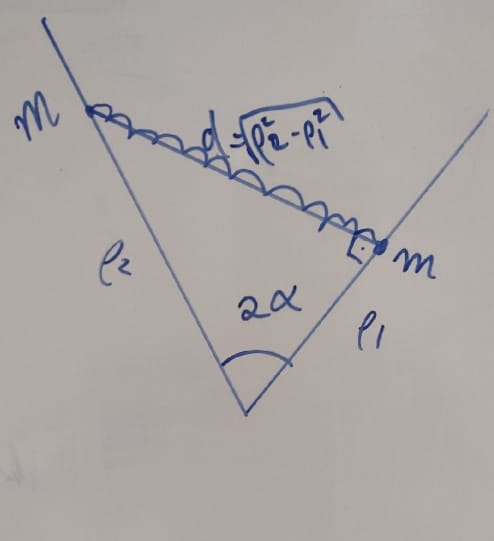
\includegraphics[width=0.5\textwidth]{perp.jpg}
\end{figure}
Como se ilustra en la Figura \ref{perp}, para que sea perpendicular a una de las barras, es necesario que distancia $D$ verifique una relación particular con las variables (de no-equilibrio):

$$D = \sqrt{\rho_2^2 - \rho_1^2}$$

Esto significa que, necesariamente, 

$$\rho_1^2 + \rho_2^2 -2\rho_1\rho_2\cos(2\alpha) = \rho_2^2 - \rho_1^2 $$

O sea,

\begin{equation}
  \label{rho1rho2}
  \rho_1 = \rho_2 \cos(2\alpha)
\end{equation}

Y, finalmente, que:

\begin{equation}
  \label{Dalt}
  D = \rho_2 \sin(2\alpha)
\end{equation}

Para resolver el problema, utilizaremos, además de las ecuaciones \eqref{rho1rho2} y \eqref{Dalt}, la conservación de energía\footnote{Que está justificado por la independencia temporal explícita del lagrangiano.} y escribiremos que, para que $v_{0}$ sea la mínima energía para que exista un punto en que sean perpendiculares las barras:

$$\frac{1}{2}m v_0^2 = \frac{1}{2}k(D^2-2l_0D)+mg\cos{\alpha}(\rho_1 + \rho_2)  = \frac{1}{2}k D^2 + kl_{0}((\rho_1 + \rho_2 )\cos(\alpha)-D)$$

Que, por nuestras expresiones, se simplificara a:
$$\frac{1}{2}m v_0^2 = \frac{1}{2}k\rho_2^2 \sin^2(2\alpha) + kl_{0}(\rho_2(\cos(2\alpha) + 1)\cos(\alpha) -\rho_2 \sin(2\alpha))$$
$$ \frac{1}{2}m v_0^2 = \rho_2^2 \left(\frac{k\sin^2(2\alpha)}{2}\right) + \rho_2\left(kl_0(\cos^3(\alpha)-\sin(2\alpha))\right) $$
De manera que tendremos, finalmente,

\begin{equation}
  \rho_2^2 \left(\frac{k\sin^2(2\alpha)}{2}\right) + \rho_2\left(kl_0(\cos^3(\alpha)-\sin(2\alpha))\right) - \frac{1}{2}m v_0^2 = 0
\end{equation}

Finalmente, tendremos que analizar para cuales $v_{0}$ el discriminante de esta ecuación cuadrática es 0, y esta será la velocidad mínima. No obstante, como $\left(\frac{k\sin^2(2\alpha)}{2}\right) \ge  0$ y  $\left(kl_0(\cos^3(\alpha)-\sin(2\alpha))\right)^{2} \ge 0$, tendremos que el discriminante ($b^2 -4ac$ para $ax^2 +bx + c$) será siempre positivo, y 0 si y solo si los otros términos son 0. De esa manera, no importa la velocidad, en algún momento tendremos una configuración en que el muelle está perpendicular a las barras.\footnote{En realidad, probamos apenas que la perpendicularidad es un estado accesible del espacio de fases a cualquier energía inicial E. Demostrar que un sistema mecánico explorará todo el espacio de fases permitido con tiempo suficiente es una cuestión un poco menos trivial.}


\subsection*{c) Se tumba el sistema de modo que exista horizontalmente, de modo que todo está contenido en el plano $xz$. Que pasa con el sistema?}

En este caso, la única diferencia será que no tendremos la presencia de la gravedad. De esta manera, lo único que va a de hecho cambiar serán las posiciones de equilibrio, ya que nuestros modos y frecuencias normales no dependen de ella. Entonces, tendremos las mismas frecuencias y modos normales, esto es:

\begin{equation}
  \begin{aligned}
  \omega_0 = \sqrt{ \frac{k}{m} (1 - \cos{2\alpha})}\\
  \omega_1 = \sqrt{ \frac{k}{m} (1 + \cos{2\alpha})}
  \end{aligned}
\end{equation}

\begin{equation}
  \begin{aligned}
  \eta_0 = \bar{\rho}_1 + \bar{\rho}_2\\
  \eta_1 = \bar{\rho}_1 - \bar{\rho}_2
  \end{aligned}
\end{equation}


Para este sistema, tendremos que el potencial será:

$$U = \frac{k}{2} (D-l_0)^{2}$$

Y por lo tanto,

$$\partial_{\rho_{1}}U = k(D-l_0)\partial_{\rho_{1}}D = 0 $$

O sea\footnote{para la solución no-trivial},
$$D = l_{0}$$

Que, con la condición de $\rho_1= \rho_2 = \rho_{eq}$, será equivalente a:

$$2\rho_{eq}^2 - 2\rho_{eq}^2 \cos{2\alpha} = 2(1-\cos{2\alpha}) \rho_{eq}^2 = l_0^2$$

\begin{equation}
\rho_{eq} = \frac{l_0}{\sqrt{2(1-\cos{2\alpha})}} = \frac{l_0}{2\sin(\alpha)}
\end{equation}

Donde lo último se ha utilizado la sencilla relación de $1-\cos{2\alpha} = 2\sin^2{\alpha}$ para simplificar. Finalmente, aunque se ha calculado la posición de equilibrio `del 0', es importante mencionar que la cantidad calculada es exactamente lo que se obtiene si tomamos $g=0$ en la ecuación \eqref{eq}, que es exactamente lo que esperamos que pase. 

Dicho de otra manera, el sistema entero es igual salvo la posición de equilibrio, que por su vez será en un punto un poco más distante del vértice, esto es, la gravedad no afecta el movimiento, solo el reposo.
 
\end{document}

